\documentclass[main-ap-physics.tex]{subfiles}

\begin{document}

\section{Kinematics}

\subsection{Displacement}

\subsubsection*{Position}

In order to describe the motion of an object, you must first be able to describe its \gls{position}---where it is at any particular time. More precisely, you need to specify its position relative to a convenient reference frame. Earth is often used as a reference frame, and we often describe the position of an object as it relates to stationary objects in that reference frame. For example, a rocket launch would be described in terms of the position of the rocket with respect to the Earth as a whole, while a professor's position could be described in terms of where she is in relation to the nearby white board. (See Figure ?.??.) In other cases, we use reference frames that are not stationary but are in motion relative to the Earth. To describe the position of a person in an airplane, for example, we use the airplane, not the Earth, as the reference frame. (See Figure ??.?.)

\subsubsection*{Displacement} \label{awplYI}

If an object moves relative to a reference frame (for example, if a professor moves to the right relative to a white board or a passenger moves toward the rear of an airplane), then the object's position changes. This change in position is known as \gls{displacement}. The word ``displacement'' implies that an object has moved, or has been displaced.

\vspace{1ex}

\begin{mdframed}[backgroundcolor=black!10]
    \textbf{Displacement}

    \vspace{1ex}
    
    Displacement is the \textit{change in position} of an object:

    \begin{equation} \label{PhLnzc}
        \Delta{x} = x_f - x_0
    \end{equation}

    where $\Delta{x}$ is displacement, $x_f$ is final position, and $x_0$ is initial position.
\end{mdframed}

In this text the upper case Greek letter $\Delta$ (delta) always means ``change in'' whatever quantity follows it; thus, $\Delta{x}$ means \textit{change in position}. Always solve for displacement by subtracting initial position  $x_0$ from final position $x_f$.

\vspace{1em}
 .
Note that the SI unit for displacement is the meter (m) (see Physical Quantities and Units), but sometimes kilometers, miles, feet, and other units of length are used. Keep in mind that when units other than the meter are used in a problem, you may need to convert them into meters to complete the calculation.

\vspace{1em} % 2 Figures

Note that displacement has a direction as well as a magnitude. The professor's displacement is \SI{2.0}{m} to the right, and the airline passenger's displacement is \SI{4.0}{m} toward the rear. In one-dimensional motion, direction can be specified with a plus or minus sign. When you begin a problem, you should select which direction is positive (usually that will be to the right or up, but you are free to select positive as being any direction). The professor's initial position is $x_0 = \SI{1.5}{m}$ and her final position is $x_f = \SI{3.5}{m}$. Thus her displacement is

\begin{equation*}
    \Delta{x} = x_f - x_0 = \SI{3.5}{m} - \SI{1.5}{m} = +\SI{2.0}{m}
\end{equation*}

In this coordinate system, motion to the right is positive, whereas motion to the left is negative. Similarly, the airplane passenger's initial position is $x_0= \SI{6.0}{m}$ and his final position is  $x_f = \SI{2.0}{m}$, so his displacement is

\begin{equation*}
    \Delta{x} = x_f - x_0 = \SI{2.0}{m} - \SI{6.0}{m} = -\SI{4.0}{m}
\end{equation*}

His displacement is negative because his motion is toward the rear of the plane, or in the negative $x$ direction in our coordinate system.

\subsubsection*{Distance}

Although displacement is described in terms of direction, distance is not. \Gls{distance} is defined to be the magnitude or size of displacement between two positions. Note that the distance between two positions is not the same as the distance traveled between them. \Gls{distance traveled} is the total length of the path traveled between two positions. Distance has no direction and, thus, no sign. For example, the distance the professor walks is \SI{2.0}{m}. The distance the airplane passenger walks is \S{4.0}{m}.

\vspace{1ex}

\begin{mdframed}[backgroundcolor=black!10]
    \textbf{Misconception Alert: distance traveled vs.~magnitude of displacement}

    \vspace{1ex}
    
    It is important to note that the distance traveled, however, can be greater than the magnitude of the displacement (by magnitude, we mean just the size of the displacement without regard to its direction; that is, just a number with a unit). For example, the professor could pace back and forth many times, perhaps walking a distance of \SI{150}{m} during a lecture, yet still end up only \SI{2.0}{m} to the right of her starting point. In this case her displacement would be $+\SI{2.0}{m}$, the magnitude of her displacement would be \SI{2.0}{m}, but the distance she traveled would be \SI{150}{m}. In kinematics we nearly always deal with displacement and magnitude of displacement, and almost never with distance traveled. One way to think about this is to assume you marked the start of the motion and the end of the motion. The displacement is simply the difference in the position of the two marks and is independent of the path taken in traveling between the two marks. The distance traveled, however, is the total length of the path taken between the two marks.
\end{mdframed}

\begin{example} \label{bcBeYE}
    A cyclist rides \SI{3}{km} west and then turns around and rides \SI{2}{km} east. (a) What is her displacement? 
\end{example}

\Solution Although we are not given initial or final positions, we are given two separate displacements. If we define east as the positive direction, and west as the negative, as shown in the figure below, then the two displacements are

\begin{equation*}
    \Delta{x_1} = -\SI{3.0}{km} \quad \text{and} \quad \Delta{x_2} = +\SI{2.0}{km}
\end{equation*}

\begin{center}
    \begin{tikzpicture}
    \begin{axis}[width=15cm,
        axis lines = left,
        axis y line=none,
        xlabel = {Position (m)},
        ymin=0, ymax=12, 
        xmin=-4, xmax=4,
        ticks=none,
        clip=false,
        ]
        \node[right] at (4,0) {E ($+x$)};
        \node[left] at (-4,0) {W ($-x$)};
        \node[above] at (0,0) {\huge \faBicycle};
        \draw[->] (0,1) node[gray,right] {$x_0$} -- ++(axis direction cs: -3,0) node[above,pos=0.5] {$\Delta{x_1} = -\SI{3.0}{km}$};
        \draw[->] (-3,1.75) -- ++(axis direction cs: 2,0) node[above,pos=0.5] {$\Delta{x_2} = +\SI{2.0}{m}$} node[gray,right] {$x_f$};
    \end{axis}
    \end{tikzpicture}
\end{center}

The total displacement is found by summing the object's individual displacements as

\begin{equation*}
    \Delta{x} = \Delta{x_1} + \Delta{x_2} = -\SI{3.0}{km} + \SI{2.0}{km} = -\SI{1.0}{km}
\end{equation*}

The cyclist's displacement is $-\SI{1.0}{km}$, or 1.0 kilometer to the west of their original position. 

\endsolution    

\vspace{1ex}

\begin{example}
   What distance does the cyclist from Example \ref{bcBeYE} ride? 
\end{example}

\Solution To find her distance traveled, we may take the sum the \textit{magnitudes} (i.e., absolute values) of each displacement:

\begin{equation*}
    \text{distance traveled} = \lvert \Delta{x_1} \rvert + \lvert \Delta{x_2} \rvert
        = \lvert -3 \rvert + \lvert 2 \rvert 
        = 3 + 2 = 5
\end{equation*}

Therefore, her total distance traveled is \SI{5.0}{km}.

\endsolution

\vspace{1ex}

\begin{example}
    What is the magnitude of the cyclist's displacement from Example \ref{bcBeYE}?
\end{example}

\Solution In Example \ref{bcBeYE}, we calculated a displacement of $\Delta{x} = -\SI{1.0}{km}$. The magnitude of this displacement is given by the absolute value:

\begin{equation*}
    \text{magnitude of displacement} = \lvert \Delta{x} \rvert = \lvert -\SI{1.0}{km} \rvert = \SI{1.0}{km}
\end{equation*}

Since taking the absolute value is effectively dropping the negative sign, the magnitude (or size) of her displacement is 1.0 kilometer.

\endsolution

\subsection{Vectors, Scalars, and Coordinate Systems} \label{1QLrzP}

What is the difference between distance and displacement? Whereas displacement is defined by both direction and magnitude, distance is defined only by magnitude. Displacement is an example of a vector quantity. Distance is an example of a scalar quantity. A \gls{vector} is any quantity with both magnitude and direction. Other examples of vectors include a velocity of \SI{90}{km/h} east and a force of \SI{500}{newtons} straight down.

\vspace{1em}

The direction of a vector in one-dimensional motion is given simply by a plus ($+$) or minus ($-$) sign. Vectors are represented graphically by arrows. An arrow used to represent a vector has a length proportional to the vector's magnitude (e.g., the larger the magnitude, the longer the length of the vector) and points in the same direction as the vector.

\vspace{1em}

Some physical quantities, like distance, either have no direction or none is specified. A \gls{scalar} is any quantity that has a magnitude, but no direction. For example, a \SI{20}{\degreeCelsius} temperature, the 250 kilocalories (250 Calories) of energy in a candy bar, a \SI{90}{km/h} speed limit, a person's 1.8 m height, and a distance of 2.0 m are all scalars—quantities with no specified direction. Note, however, that a scalar can be negative, such as a  \SI{-20}{\degreeCelsius} temperature. In this case, the minus sign indicates a point on a scale rather than a direction. Scalars are never represented by arrows.

\subsubsection*{Coordinate Systems for One-Dimensional Motion}

In order to describe the direction of a vector quantity, you must designate a coordinate system within the reference frame. For one-dimensional motion, this is a simple coordinate system consisting of a one-dimensional coordinate line. In general, when describing horizontal motion, motion to the right is usually considered positive, and motion to the left is considered negative. With vertical motion, motion up is usually positive and motion down is negative. In some cases, however, as with the jet in Figure ?.?, it can be more convenient to switch the positive and negative directions. For example, if you are analyzing the motion of falling objects, it can be useful to define downwards as the positive direction. If people in a race are running to the left, it is useful to define left as the positive direction. It does not matter as long as the system is clear and consistent. Once you assign a positive direction and start solving a problem, you cannot change it.

\begin{center}
    \begin{tikzpicture}
        \begin{axis}[width=4cm,
            height=4cm,
            xmin=-1,xmax=1,
            ymin=-1,ymax=1,
            ticks=none,
            axis line style={draw=none},
            clip=false
            ]
            \draw[<->] (-1,0) node[left] {$-x$} -- (1,0) node[right] {$+x$};
            \draw[<->] (0,-1) node[below] {$-y$} -- (0,1) node[above] {$+y$};
        \end{axis}
    \end{tikzpicture}
\end{center}

\begin{example}
    A person's speed can stay the same as they round a corner and changes direction. Given this information, is speed a scalar or a vector quantity? Explain.
\end{example}

\Solution Speed is a scalar quantity. It does not change at all with direction changes; therefore, it has magnitude only. If it were a vector quantity, it would change as direction changes (even if its magnitude remained constant).

\endsolution

\subsection{Time, Velocity, and Speed} \label{3hdww6}

There is more to motion than distance and displacement. Questions such as, ``How long does a foot race take?'' and ``What was the runner's speed?'' cannot be answered without an understanding of other concepts. In this section we add definitions of time, velocity, and speed to expand our description of motion.

\subsubsection*{Time}

As discussed in [Physical Quantities and Units], the most fundamental physical quantities are defined by how they are measured. This is the case with time. Every measurement of time involves measuring a change in some physical quantity. It may be a number on a digital clock, a heartbeat, or the position of the Sun in the sky. In physics, the definition of time is simple---\gls{time} is \textit{change}, or the interval over which change occurs. It is impossible to know that time has passed unless something changes.

\vspace{1em}

The amount of time or change is calibrated by comparison with a standard. The SI unit for time is the second, abbreviated s. We might, for example, observe that a certain pendulum makes one full swing every \SI{0.75}{s}. We could then use the pendulum to measure time by counting its swings or, of course, by connecting the pendulum to a clock mechanism that registers time on a dial. This allows us to not only measure the amount of time, but also to determine a sequence of events.

\vspace{1em}

How does time relate to motion? We are usually interested in elapsed time for a particular motion, such as how long it takes an airplane passenger to get from his seat to the back of the plane. To find elapsed time, we note the time at the beginning and end of the motion and subtract the two. For example, a lecture may start at 11:00 A.M. and end at 11:50 A.M., so that the elapsed time would be 50 min. \gls{elapsed time} ${\Delta}t$ is the difference between the ending time and beginning time,

\begin{equation*}
    \Delta t = t_f = t_0
\end{equation*}

where $\Delta t$ is the change in time or elapsed time, $t_f$ is the time at the end of the motion, and $t_0$ is the time at the beginning of the motion. (As usual, the delta symbol, $\Delta$, means the change in the quantity that follows it.)

\vspace{1em}

Life is simpler if the beginning time $t_0$ is taken to be zero, as when we use a stopwatch. If we were using a stopwatch, it would simply read zero at the start of the lecture and \SI{50}{min} at the end. If $t_0 = 0$, then $\Delta t = t_f \equiv t$.

\vspace{1em}

In this text, for simplicity’s sake,

\begin{itemize}
\setlength\itemsep{0.1ex}
    \item motion starts at time equal to zero ($t_0 = 0$)
    \item the symbol $t$ is used for elapsed time unless otherwise specified ($\Delta t = t_f \equiv t$)
\end{itemize}

\subsubsection*{Velocity}

Your notion of velocity is probably the same as its scientific definition. You know that if you have a large displacement in a small amount of time you have a large velocity, and that velocity has units of distance divided by time, such as miles per hour or kilometers per hour.

\begin{mdframed}[backgroundcolor=black!10]
    \Gls{average velocity} is displacement (change in position) divided by the time of travel,

    \begin{equation} \label{yHaY2u}
        \bar{v} = \frac{\Delta x}{\Delta t} = \frac{x_f - x_0}{t_f - t_0}
    \end{equation}

    where $\bar{v}$ is the average (indicated by the bar over the $v$) velocity, $\Delta x$ is the change in position (or displacement), and $x_f$ and $x_0$ are the final and beginning positions at times $t_f$ and $t_0$, respectively. If the starting time $t_0$ is taken to be zero, then the average velocity is simply

    \begin{equation} \label{x7GvGS}
        \bar{v} = \frac{\Delta x}{t}
    \end{equation}
\end{mdframed}

Notice that this definition indicates that velocity is a vector because displacement is a vector. It has both magnitude and direction. The SI unit for velocity is meters per second or m/s, but many other units, such as km/h, mi/h (also written as mph), and cm/s, are in common use. Suppose, for example, an airplane passenger took 5 seconds to move $-\SI{4}{m}$ (the negative sign indicates that displacement is toward the \textit{back} of the plane). His average velocity would, by Equation \eqref{x7GvGS}, be

\begin{equation*}
    \bar{v} = \frac{\Delta x}{t} = \frac{-\SI{4}{m}}{\SI{5}{s}} = -\SI{0.8}{m/s}
\end{equation*}

The minus sign indicates the average velocity is also toward the rear of the plane.

\vspace{1em}

The average velocity of an object does not tell us anything about what happens to it between the starting point and ending point, however. For example, we cannot tell from average velocity whether the airplane passenger stops momentarily or backs up before he goes to the back of the plane. To get more details, we must consider smaller segments of the trip over smaller time intervals.

\vspace{1em} %Figure

The smaller the time intervals considered in a motion, the more detailed the information. When we carry this process to its logical conclusion, we are left with an infinitesimally small interval. Over such an interval, the average velocity becomes the instantaneous velocity or the velocity at a specific instant. A car’s speedometer, for example, shows the magnitude (but not the direction) of the instantaneous velocity of the car. (Police give tickets based on instantaneous velocity, but when calculating how long it will take to get from one place to another on a road trip, you need to use average velocity.) \gls{instantaneous velocity} $v$ is the average velocity at a specific instant in time (or over an infinitesimally small time interval).

\vspace{1em}

Mathematically, finding instantaneous velocity, $v$, at a precise instant $t$ can involve taking a limit, a calculus operation beyond the scope of this text. However, under many circumstances, we can find precise values for instantaneous velocity without calculus.

\subsubsection*{Speed}

In everyday language, most people use the terms ``speed'' and ``velocity'' interchangeably. In physics, however, they do not have the same meaning and they are distinct concepts. One major difference is that speed has no direction. Thus speed is a scalar. Just as we need to distinguish between instantaneous velocity and average velocity, we also need to distinguish between instantaneous speed and average speed.

\vspace{1em}

\Gls{instantaneous speed} is the magnitude of instantaneous velocity. For example, suppose the airplane passenger at one instant had an instantaneous velocity of $-\SI{3.0}{m/s}$ (the minus meaning toward the rear of the plane). At that same time his instantaneous speed was \SI{3.0}{m/s}. Or suppose that at one time during a shopping trip your instantaneous velocity is \SI{40}{km/h} due north. Your instantaneous speed at that instant would be \SI{40}{km/h}---the same magnitude but without a direction. Average speed, however, is very different from average velocity. \gls{average speed} is the distance traveled divided by elapsed time.

\vspace{1em}

We have noted that distance traveled can be greater than the magnitude of displacement. So average speed can be greater than average velocity, which is displacement divided by time. For example, if you drive to a store and return home in half an hour, and your car’s odometer shows the total distance traveled was \SI{6}{km}, then your average speed was \SI{12}{km/h}. Your average velocity, however, was zero, because your displacement for the round trip is zero. (Displacement is change in position and, thus, is zero for a round trip.) Thus average speed is \textit{not} simply the magnitude of average velocity.

\vspace{1em} %Figure

Another way of visualizing the motion of an object is to use a graph. A plot of position or of velocity as a function of time can be very useful. For example, for this trip to the store, the position, velocity, and speed-vs.-time graphs are displayed in Figure ?.??. (Note that these graphs depict a very simplified \gls{model} of the trip. We are assuming that speed is constant during the trip, which is unrealistic given that we’ll probably stop at the store. But for simplicity’s sake, we will model it with no stops or changes in speed. We are also assuming that the route between the store and the house is a perfectly straight line.)

\begin{center}
    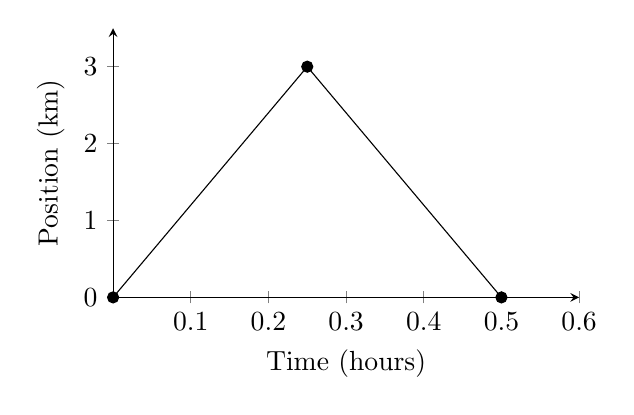
\begin{tikzpicture}
        \begin{axis}[width=7.5cm,height=5cm,
            axis lines=left,
            xmin=0,xmax=0.6,
            ymin=0,ymax=3.5,
            clip=false,
            xlabel={Time (hours)},
            ylabel={Position (km)},
            xtick={0.1,0.2,...,0.6}
        ]
        \addplot[%color=black,
            mark=*,
            ]
            coordinates {
            (0,0)(0.25,3)(0.5,0)
            };        
        \end{axis}
    \end{tikzpicture}

    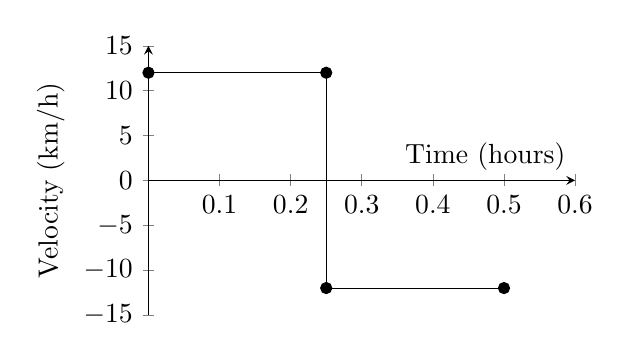
\begin{tikzpicture}
        \begin{axis}[width=7cm,height=5cm,
            axis y line=left,
            axis x line=center,
            xmin=0,xmax=0.6,
            ymin=-15,ymax=15,
            clip=false,
            ylabel={Velocity (km/h)},
            xlabel={Time (hours)},
            ytick={-15,-10,...,15},
            xtick={0.1,0.2,...,0.6}
        ]
        % \node[right=2mm] at (0.6,0) {Time (hours)};
        \addplot[%color=black,
            mark=*,
            ]
            coordinates {
            (0,12)(0.25,12)(0.25,-12)(0.5,-12)
            };
        \end{axis}
    \end{tikzpicture}

    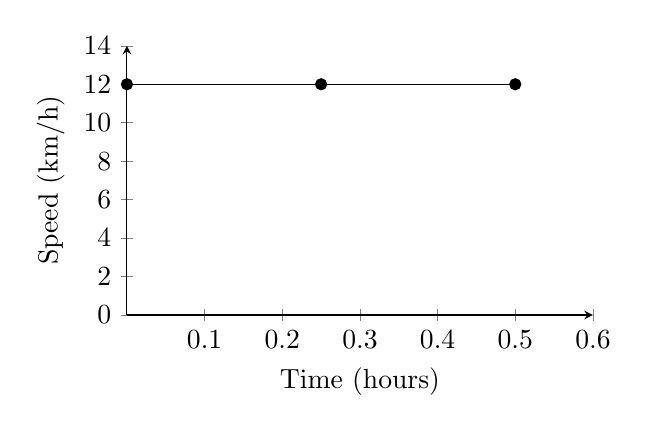
\begin{tikzpicture}
        \begin{axis}[width=7.5cm,height=5cm,
            axis lines=left,
            xmin=0,xmax=0.6,
            ymin=0,ymax=14,
            clip=false,
            xlabel={Time (hours)},
            ylabel={Speed (km/h)},
            xtick={0.1,0.2,...,0.6},
            ytick={0,2,...,14}
        ]
        \addplot[%color=black,
            mark=*,
            ]
            coordinates {
            (0,12)(0.25,12)(0.5,12)
            };        
        \end{axis}
    \end{tikzpicture}
\end{center}

\begin{mdframed}[backgroundcolor=black!10]
    If you have spent much time driving, you probably have a good sense of speeds between about 10 and 70 miles per hour. But what are these in meters per second? What do we mean when we say that something is moving at \SI{10}{m/s}? To get a better sense of what these values really mean, do some observations and calculations on your own:

    \begin{itemize}
    \setlength\itemsep{0.1ex}
        \item calculate typical car speeds in meters per second
        \item estimate jogging and walking speed by timing yourself; convert the measurements into both m/s and mi/h
        \item determine the speed of an ant, snail, or falling leaf
    \end{itemize}
\end{mdframed}

\begin{example} \label{au4Ac2}
    A commuter train travels from Baltimore to Washington, DC, and back in 1 hour and 45 minutes. The distance between the two stations is approximately 40 miles. What is the average velocity of the train?
\end{example}

\Solution The average velocity of the train is zero because $x_ f= x_0$; the train ends up at the same place it starts. 

\endsolution

\begin{example}
    What is the average speed, in meters per second, of the train from Example \ref{au4Ac2}?
\end{example}

\Solution The train travels 40 miles one way and 40 miles back, so we are given a total distance of 80 miles. Also, a time of 1 hour and 45 minutes is equivalent to 105 minutes. Average speed is given by

\begin{equation*}
    \text{average speed} = \frac{\text{distance}}{\text{time}} = \frac{\text{80 miles}}{\text{105 minutes}}
\end{equation*}

We convert miles per minutes to meters per second using dimensional analysis as follows:

\begin{equation*}
    \frac{\text{80 miles}}{\text{105 minutes}}
    \times \frac{\text{5280 feet}}{\text{1 mile}}
    \times \frac{\text{1 meter}}{\text{3.28 feet}}
    \times \frac{\text{1 minute}}{\text{60 seconds}} = \SI{20}{m/s}
\end{equation*}

\subsection{Acceleration} \label{LgXYss}

% Figure

In everyday conversation, to accelerate means to speed up. The accelerator in a car can in fact cause it to speed up. The greater the acceleration, the greater the change in velocity over a given time. The formal definition of acceleration is consistent with these notions, but more inclusive.

\begin{mdframed}[backgroundcolor=black!10]
    Average Acceleration is the rate at which velocity changes,

    \begin{equation} \label{vdyjX5}
        \bar{a} = \frac{\Delta v}{\Delta t} = \frac{v_f - v_0}{t_f - t_0} 
    \end{equation}

    where $\bar{a}$ is average acceleration, $v$ is velocity, and $t$is time. (The bar over the $a$ means average acceleration.)
\end{mdframed}

Because acceleration is velocity in m/s divided by time in s, the SI units for acceleration are \SI{}{m/s^2}, meters per second squared or meters per second per second, which literally means by how many meters per second the velocity changes every second.

\vspace{1em}

Recall that velocity is a vector---it has both magnitude and direction. This means that a change in velocity can be a change in magnitude (or speed), but it can also be a change in direction. For example, if a car turns a corner at constant speed, it is accelerating because its direction is changing. The quicker you turn, the greater the acceleration. So there is an acceleration when velocity changes either in magnitude (an increase or decrease in speed) or in direction, or both.

\begin{mdframed}[backgroundcolor=black!10]
    \textbf{Acceleration as a vector}

    \vspace{1ex}

    Acceleration is a vector in the same direction as the change in velocity, $\Delta v$. Since velocity is a vector, it can change either in magnitude or in direction. Acceleration is therefore a change in either speed or direction, or both.
\end{mdframed}

Keep in mind that although acceleration is in the direction of the change in velocity, it is not always in the direction of motion. When an object slows down, its acceleration is opposite to the direction of its motion. This is known as \gls{deceleration}.

\vspace{1em} % Figure

\begin{mdframed}[backgroundcolor=yellow!10]
    \textbf{Misconception alert: Deceleration vs.~negative acceleration}

    \vspace{1ex}

    Deceleration always refers to acceleration in the direction opposite to the direction of the velocity. Deceleration always reduces speed. Negative acceleration, however, is acceleration \textit{in the negative direction in the chosen coordinate system}. Negative acceleration may or may not be deceleration, and deceleration may or may not be considered negative acceleration. For example, consider Figure ?.??

    \begin{center}
        \begin{tikzpicture}
            \begin{axis}[width=8cm,height=2.5cm,
                xmin=2,xmax=8,
                ymin=0,ymax=12,
                ticks=none,
                axis line style={draw=none}, 
                clip=false,
            ]
                \node at (4,0) {\mycar};
                \draw (6,0) node[left=-3mm] {\textcolor{black!15}{\mycar}}
                node[left=-5mm] {\textcolor{black!30}{\mycar}}
                node {\mycar};
                \draw[->] (3.5,12) -- ++(axis direction cs: 2,0) node[right] {$v$} node[above=2mm,pos=0.5] {(a) Speeding Up};
                \draw[->] (4,8) -- ++(axis direction cs: 1,0) node[right] {$a$};
            \end{axis}
        \end{tikzpicture}%
        \hspace{1cm}
        \begin{tikzpicture}
            \begin{axis}[width=8cm,height=2.5cm,
                xmin=2,xmax=8,
                ymin=0,ymax=12,
                ticks=none,
                axis line style={draw=none}, 
                clip=false,
            ]
                \node at (6,0) {\mycar};
                \draw (4,0) node[left=-3mm] {\textcolor{black!15}{\mycar}}
                node[left=-5mm] {\textcolor{black!30}{\mycar}}
                node {\mycar};
                \draw[->] (3.5,12) -- ++(axis direction cs: 2,0) node[right] {$v$} node[above=2mm,pos=0.5] {(b) Slowing Down};
                \draw[<-] (4,8) -- ++(axis direction cs: 1,0) node[right] {$a$};
            \end{axis}
        \end{tikzpicture}

        \vspace{2em}

        \begin{tikzpicture}
            \begin{axis}[width=8cm,height=2.5cm,
                xmin=2,xmax=8,
                ymin=0,ymax=12,
                ticks=none,
                axis line style={draw=none}, 
                clip=false,
            ]
                \node at (4,0) {\mycarleft};
                \draw (6,0) node[right=-1.5mm] {\textcolor{black!15}{\mycarleft}}
                node[right=-3.5mm] {\textcolor{black!30}{\mycarleft}}
                node {\mycarleft};
                \draw[<-] (3.5,12) -- ++(axis direction cs: 2,0) node[right] {$v$} node[above=2mm,pos=0.5] {(c) Slowing Down};
                \draw[->] (4,8) -- ++(axis direction cs: 1,0) node[right] {$a$};
            \end{axis}
        \end{tikzpicture}%
        \hspace{1cm}
        \begin{tikzpicture}
            \begin{axis}[width=8cm,height=2.5cm,
                xmin=2,xmax=8,
                ymin=0,ymax=12,
                ticks=none,
                axis line style={draw=none}, 
                clip=false,
            ]
                \node at (6,0) {\mycarleft};
                \draw (4,0) node[right=-1.5mm] {\textcolor{black!15}{\mycarleft}}
                node[right=-3.5mm] {\textcolor{black!30}{\mycarleft}}
                node {\mycarleft};
                \draw[<-] (3.5,12) -- ++(axis direction cs: 2,0) node[right] {$v$} node[above=2mm,pos=0.5] {(d) Speeding Up};
                \draw[<-] (4,8) -- ++(axis direction cs: 1,0) node[right] {$a$};
            \end{axis}
        \end{tikzpicture}
        \captionsetup{type=figure,margin=1in,font=scriptsize}
        \captionof{figure}{(a) This car is speeding up as it moves toward the right. It therefore has positive acceleration in our coordinate system. (b) This car is slowing down as it moves toward the right. Therefore, it has negative acceleration in our coordinate system, because its acceleration is toward the left. The car is also decelerating: the direction of its acceleration is opposite to its direction of motion. (c) This car is moving toward the left, but slowing down over time. Therefore, its acceleration is positive in our coordinate system because it is toward the right. However, the car is decelerating because its acceleration is opposite to its motion. (d) This car is speeding up as it moves toward the left. It has negative acceleration because it is accelerating toward the left. However, because its acceleration is in the same direction as its motion, it is speeding up (not decelerating).}
    \end{center}
\end{mdframed}

\begin{example}
    A racehorse coming out of the gate accelerates from rest to a velocity of \SI{15.0}{m/s} due west in \SI{1.80}{s}. What is its average acceleration?
\end{example}

\Solution First we draw a sketch and assign a coordinate system to the problem. This is a simple problem, but it always helps to visualize it. Notice that we assign east as positive and west as negative. Thus, in this case, we have negative velocity.

\begin{center}
    \begin{tikzpicture}
        \begin{axis}[width=4cm,
            height=4cm,
            xmin=-1,xmax=1,
            ymin=-1,ymax=1,
            ticks=none,
            axis line style={draw=none},
            clip=false
            ]
            
            \draw[<->] (-1,0) node[left] {W ($-x$)} -- (1,0) node[right] {E ($+x$)};
            \draw[<->] (0,-1) node[below] {S ($-y$)} -- (0,1) node[above] {N ($+y$)};

            \begin{scope}[shift={(axis direction cs: -4,0)}]
                \draw[fill=black] (0,0) circle (2pt) node[below]{$v_0 = 0$};
                \draw[thick,->] (-1.5,0) -- ++(axis direction cs: -3,0) node[pos=0.5,below] {$v_f = -\SI{15}{m/s}$}; 
                \draw[Green,thick,->] (-0.5,0.8) -- ++(axis direction cs: -2,0) node[pos=0.5,above] {$a =\ ?$};
                
            \end{scope}
        \end{axis}
    \end{tikzpicture}
\end{center}

We are given initial velocity (``from rest''), final velocity, and elapsed time: $v_0 = 0$, $v_f = -\SI{15}{m/s}$, and $\Delta{t} = \SI{1.80}{s}$. (The negative sign on $v_f$ indicates direction toward the west.)

\vspace{1em}

The unknown we are looking for is acceleration: $a =\ ?$ By Equation \eqref{vdyjX5}, average acceleration is

\begin{equation*}
    \bar{a} = \frac{\Delta{v}}{\Delta{t}}
\end{equation*}

where the horse's change in velocity is

\begin{equation*}
    \Delta{v} = v_f - v_0 = -\SI{15}{m/s} - 0 = \SI{-15}{m/s}
\end{equation*}

Therefore, the average acceleration is

\begin{equation*}
    \bar{a} = \frac{\Delta v}{\Delta t} = \frac{-\SI{15}{m/s}}{\SI{1.80}{s}} = -\SI{8.33}{m/s^2}
\end{equation*}

The negative sign for acceleration indicates that acceleration is toward the west. An acceleration of \SI{8.33}{m/s^2} due west means that the horse increases its velocity by \SI{8.33}{m/s} due west each second, that is, 8.33 meters per second per second, which we write as \SI{8.33}{m/s^2}. This is truly an average acceleration, because the ride is not smooth. We shall see later that an acceleration of this magnitude would require the rider to hang on with a force nearly equal to his weight.

\endsolution

\Gls{instantaneous acceleration} $a$, or the \textit{acceleration at a specific instant in time}, is obtained by the same process as discussed for instantaneous velocity in \nameref{3hdww6}---that is, by considering an infinitesimally small interval of time. How do we find instantaneous acceleration using only algebra? The answer is that we choose an average acceleration that is representative of the motion. Figure \ref{6040uO} shows graphs of instantaneous acceleration versus time for two very different motions. In Figure \ref{6040uO}(a), the acceleration varies slightly and the average over the entire interval is nearly the same as the instantaneous acceleration at any time. In this case, we should treat this motion as if it had a constant acceleration equal to the average (in this case about \SI{1.8}{m/s^2}). In Figure \ref{6040uO}(b), the acceleration varies drastically over time. In such situations it is best to consider smaller time intervals and choose an average acceleration for each. For example, we could consider motion over the time intervals from 0 to \SI{1.0}{s} and from 1.0 to \SI{3.0}{s} as separate motions with accelerations of $+\SI{3.0}{m/s^2}$ and $-\SI{2.0}{m/s^2}$, respectively.

\begin{center}
\begin{minipage}{7cm}
    \centering
    \begin{tikzpicture}
        \begin{axis}[width=6cm, height=3cm,
            xmin=0,xmax=5,
            ymin=0,ymax=2,
            xtick={0,1,...,5},
            ytick={0,1,2},
            xlabel={$t$ (s)},
            ylabel={$a$ (\SI{}{m/s^2})},
            axis lines=center,
            y label style={at={(axis description cs:0,1)},above=2mm},
            x label style={at={(axis description cs:1,0.0)},right=2mm},
            clip=false,
            ]
            \draw[thick,Green] plot[,domain=0:5,variable=\x,samples=100] (\x,{0.5*sin(125*\x) + 1.8});
            \draw[thick,dashed] (0,1.8) -- ++(axis direction cs: 5,0) node[pos=1.1,above] {$\bar{a} = \text{average}$};
        \end{axis}
    \end{tikzpicture}
    
    \vspace{2em}
    (a)
\end{minipage}%
\begin{minipage}{7cm}
    \centering
    \begin{tikzpicture}
        \begin{axis}[width=6cm,height=6cm,
            axis lines=left,
            xmin=0,xmax=6.5,
            ymin=-5,ymax=5,
            xtick={0,1,...,6},
            ytick={-5,-4,...,5},
            axis lines = center,
            xlabel={$t$ (s)},
            ylabel={$a$ (\SI{}{m/s^2})},
            y label style={at={(axis description cs:0,1)},above=2mm},
            x label style={at={(axis description cs:1,0.5)},right=2mm},
        ]
        \addplot[Green,mark=none,thick]
            coordinates{
                (0,3)(1,3)(1,-2)(3,-2)(3,0)(4.2,0)(4.2,1)(4.9,1)
                (4.9,5)(5.5,5)(5.5,-4)(6,-4)(6,-1.5)
            };
        \end{axis}
    \end{tikzpicture}
    
    (b)
\end{minipage}%
\end{center}
\captionsetup{type=figure,margin=1in,font=scriptsize}
\captionof{figure}{Graphs of instantaneous acceleration versus time for two different one-dimensional motions. (a) Here acceleration varies only slightly and is always in the same direction, since it is positive. The average over the interval is nearly the same as the acceleration at any given time. (b) Here the acceleration varies greatly, perhaps representing a package on a post office conveyor belt that is accelerated forward and backward as it bumps along. It is necessary to consider small time intervals (such as from 0 to \SI{1.0}{s}) with constant or nearly constant acceleration in such a situation.}
\label{6040uO}

The next several examples consider the motion of the subway train shown in Figure \ref{GMa3RN}. In (a) the shuttle moves to the right, and in (b) it moves to the left. The examples are designed to further illustrate aspects of motion and to illustrate some of the reasoning that goes into solving problems.

\begin{center}
    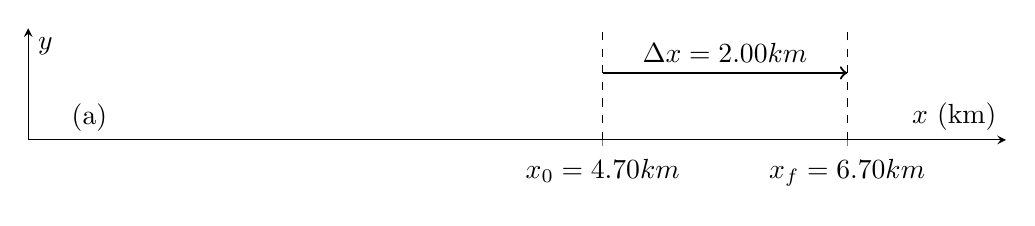
\begin{tikzpicture}
        \begin{axis}[width=14cm,
            height=3cm,
            ymin=0,ymax=10,
            xmin=0,xmax=8,
            axis lines=center,
            ylabel=$y$,
            xlabel=$x$ (km),
            %ticks=none,
            ytick=\empty,
            clip=false,
            xtick={4.7, 6.7}, 
            xticklabels = {\strut $x_0=\SI{4.70}{km}$, \strut $x_f = \SI{6.70}{km}$}, 
            ]
            \draw (4.7,0) node[above left] {\mytrain};
            \draw (0.5,2) node {(a)};
            \draw[dashed] (4.7,0) -- ++(axis direction cs: 0,10);
            \draw[dashed] (6.7,0) -- ++(axis direction cs: 0,10);
            \draw[thick,->] (4.7,6) -- ++(axis direction cs: 2,0) node[pos=0.5,above] {$\Delta x = \SI{2.00}{km}$};
        \end{axis}
    \end{tikzpicture}

    \vspace{1em}
    
    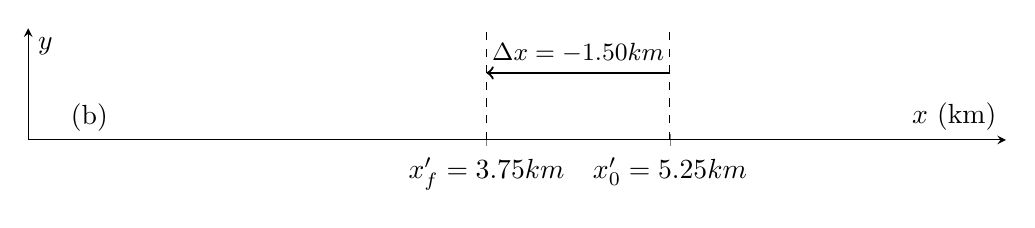
\begin{tikzpicture}
        \begin{axis}[width=14cm,
            height=3cm,
            ymin=0,ymax=10,
            xmin=0,xmax=8,
            axis lines=center,
            ylabel=$y$,
            xlabel=$x$ (km),
            %ticks=none,
            ytick=\empty,
            clip=false,
            xtick={3.75, 5.25}, 
            xticklabels = {\strut $x_f^{\prime}=\SI{3.75}{km}$, \strut $x_0^{\prime} = \SI{5.25}{km}$}, 
            ]
            \draw (5.25,0) node[above right] {\mytrainleft};
            \draw (0.5,2) node {(b)};
            \draw[dashed] (3.75,0) -- ++(axis direction cs: 0,10);
            \draw[dashed] (5.25,0) -- ++(axis direction cs: 0,10);
            \draw[thick,->] (5.25,6) -- ++(axis direction cs: -1.5,0) node[pos=0.5,above] {\small $\Delta x = -\SI{1.50}{km}$};
        \end{axis}
    \end{tikzpicture}
\captionsetup{type=figure,margin=1in,font=scriptsize}
\captionof{figure}{One-dimensional motion of a subway train considered in the Examples below. Here we have chosen the $x$ axis so that $+$ means to the right and $-$ means to the left for displacements, velocities, and accelerations. (a) The subway train moves to the right from $x_0$ to $x_f$. Its displacement $\Delta x$ is $+\SI{2.0}{km}$. (b) The train moves to the left from $x_0^{\prime}$ to $x_f^{\prime}$. Its displacement $\Delta x^{\prime}$ is $-\SI{1.50}{km}$. (Note that the prime symbol ($\prime$) is used simply to distinguish between displacement in the two different situations. The distances of travel and the size of the cars are on different scales to fit everything into the diagram.)}
\label{GMa3RN}
\end{center}

\begin{example} \label{Zg8Ig4}
    \textit{Calculating Displacement: A Subway Train}. What are the magnitude and sign of displacements for the motions of the subway train shown in parts (a) and (b) of Figure \ref{GMa3RN}.
\end{example}

\Solution Our strategy: A drawing with a coordinate system is already provided, so we don't need to make a sketch, but we should analyze it to make sure we understand what it is showing. Pay particular attention to the coordinate system. To find displacement, we use Equation \eqref{PhLnzc}, $\Delta{x} = x_f - x_0$. This is straightforward since the initial and final positions are given.

\vspace{1em}

We are given the initial and final positions for both parts:

\begin{equation*}
    x_f = \SI{6.70}{km}\ ,\ x_0=\SI{4.70}{km} \quad
    \text{and} \quad
    x_f^{\prime}=\SI{3.75}{km}\ ,\ x_0^{\prime} = \SI{5.25}{km}
\end{equation*}

Therefore, the displacements are

\begin{equation*}
    \Delta x = x_f - x_0 = \SI{6.70}{km} - \SI{4.70}{km} = +\SI{2.00}{km}
\end{equation*}

and

\begin{equation*}
    \Delta x^{\prime} = x_f^{\prime} - x_0^{\prime} = \SI{3.75}{km} - \SI{5.25}{km} = -\SI{1.50}{km}
\end{equation*}

The direction of the motion in (a) is to the right and therefore its displacement has a positive sign, whereas motion in (b) is to the left and thus has a negative sign.

\endsolution

\begin{example}
    \textit{Comparing Distance Traveled with Displacement: A Subway Train}. What are the distances traveled for the motions shown in parts (a) and (b) of the subway train in Figure \ref{GMa3RN}?
\end{example}

\Solution To answer this question, think about the definitions of distance and distance traveled, and how they are related to displacement. Distance between two positions is defined to be the magnitude of displacement, which was found in Example \ref{Zg8Ig4}. Distance traveled is the total length of the path traveled between the two positions. (See \nameref{awplYI}.) In the case of the subway train shown in Figure \ref{GMa3RN}, the distance traveled is the same as the distance between the initial and final positions of the train.

\vspace{1em}

The displacement for part (a) was $+\SI{2.00}{km}$. Therefore, the distance between the initial and final positions was \SI{2.00}{km}, and the distance traveled was \SI{2.00}{km}.

\vspace{1em}

The displacement for part (b) was $-\SI{1.5}{km}$. Therefore, the distance between the initial and final positions was \SI{1.50}{km}, and the distance traveled was \SI{1.50}{km}.

\vspace{1em}

Distance is a scalar. It has magnitude but no sign to indicate direction.

\endsolution

\begin{example} \label{PLCGFI}
    \textit{Calculating Acceleration: A Subway Train Speeding Up}. Suppose the train in Figure \ref{GMa3RN}(a) accelerates from rest to \SI{30.0}{km/h} in the first \SI{20.0}{s} of its motion. What is its average acceleration during that time interval?
\end{example}

\Solution It is worth it at this point to make a simple sketch:

\begin{center}
    \begin{tikzpicture}
        \begin{axis}[width=4cm,
            height=4cm,
            xmin=0,xmax=2,
            ymin=0,ymax=2,
            ticks=none,
            axis line style={draw=none},
            clip=false
            ]
            
            \draw[thick,->] (0,0) -- (1,0) node[right] {$x$};
            \draw[thick,->] (0,0) -- (0,1) node[above] {$y$};

            \begin{scope}[shift={(axis direction cs: -6,1)}]
                \draw[fill=black] (0,0.5) circle (2pt) node[below=2pt]{$v_0 = \SI{0}{km/h}$};
                \draw (0,-0.5) node {\large \StopWatchStart} node[below=3mm] {\SI{0.0}{s}};
                \draw[thick,->] (1.5,0.5) -- ++(axis direction cs: 3,0) node[pos=0.5,below=2pt] {$v_f = \SI{30}{km/h}$}; 
                \draw (3,-0.5) node {\large \StopWatchEnd} node[below=3mm] {\SI{20.0}{s}};
                \draw[Green,very thick,->] (0,-1.7) -- ++(axis direction cs: 3,0) node[pos=0.5,above] {$a =\ ?$};
            \end{scope}
        \end{axis}
    \end{tikzpicture}
\end{center}

This problem involves three steps. First we must determine the change in velocity, then we must determine the change in time, and finally we use these values to calculate the acceleration.

\vspace{1em}

We are given the initial velocity, final velocity, and elapsed time: $v_0 = 0$ (the train starts at rest), $v_f = \SI{30}{km/h}$, and $\Delta t = \SI{20.0}{s}$. The train's change in velocity is

\begin{equation*}
    \Delta v = v_f - v_0 = +\SI{30}{km/h}
\end{equation*}

where the plus sign means velocity to the right. This change is exactly what we expected since it starts from rest. Average acceleration, by Equation \eqref{vdyjX5}, is

\begin{equation*}
    \bar{a} = \frac{\Delta v}{\Delta t} = \frac{+\SI{30}{km/h}}{\SI{20.0}{s}}
\end{equation*}

Since the units are mixed (we have both hours and seconds for time), we need to convert everything into SI units of meters and seconds. (See \nameref{3vggy3} for more guidance.) 

\begin{equation*}
    \bar{a} = \left(\frac{+\SI[per-mode=fraction]{30}{\kilo\meter\per\hour}}{\SI{20.0}{s}}\right)
        \left(\frac{10^3\,\text{m}}{\SI{1}{km}}\right)\left(\frac{\SI{1}{h}}{\SI{3600}{s}}\right) = +\SI{0.417}{m/s^2}
\end{equation*}

The plus sign means that acceleration is to the right. This is reasonable because the train starts from rest and ends up with a velocity to the right (also positive). So acceleration is in the same direction as the \textit{change} in velocity, as is always the case.

\endsolution

\begin{example} \label{dHBSwG}
    \textit{Calculate Acceleration: A Subway Train Slowing Down}. Now suppose that at the end of its trip, the train in Figure \ref{}(a) slows to a stop from a speed of \SI{30.0}{km/h} in \SI{8.00}{s}. What is its average acceleration while stopping?
\end{example}

\begin{center}
    \begin{tikzpicture}
        \begin{axis}[width=4cm,
            height=4cm,
            xmin=0,xmax=2,
            ymin=0,ymax=2,
            ticks=none,
            axis line style={draw=none},
            clip=false
            ]
            
            \draw[thick,->] (0,0) -- (1,0) node[right] {$x$};
            \draw[thick,->] (0,0) -- (0,1) node[above] {$y$};

            \begin{scope}[shift={(axis direction cs: -6.5,1)}]
                \draw[thick,->] (0,0.5) node[below=2pt]{$v_0 = \SI{30}{km/h}$} -- ++(axis direction cs: 3,0);
                \draw (0,-0.5) node {\large \StopWatchStart} node[below=3mm] {\SI{0.0}{s}};
                \fill (4.5,0.5) circle (2pt) node[below=2pt] {$v_f = \SI{0}{km/h}$}; 
                \draw (4.5,-0.5) node {\large \StopWatchEnd} node[below=3mm] {\SI{8.00}{s}};
                \draw[Green,very thick,<-] (0.5,-1.7) -- ++(axis direction cs: 4,0) node[pos=0.5,above] {$a =\ ?$};
            \end{scope}
        \end{axis}
    \end{tikzpicture}
\end{center}

\Solution In this case, the train is decelerating and its acceleration is negative because it is toward the left. As in the previous example, we must find the change in velocity and the change in time and then solve for acceleration.

\vspace{1em}

We are given initial velocity, final velocity, and elapsed time: $v_0 = \SI{30}{km/h}$, $v_f = 0$ (the train is stopped, so its velocity is 0), and $\Delta t = \SI{8.00}{s}$. The train's change in velocity is

\begin{equation*}
    \Delta v = v_f - v_0 = 0 - \SI{30}{km/h} = -\SI{30}{km/h}
\end{equation*}

Substituting given values into Equation \ref{vdyjX5}, for average acceleration, leads to 

\begin{equation*}
    \bar{a} = \frac{\Delta v}{\Delta t} = \frac{-\SI{30}{km/h}}{\SI{8.00}{s}}
\end{equation*}

To convert the units to meters and seconds, we compute the following:

\begin{equation*}
    \bar{a} = \left(\frac{-\SI[per-mode=fraction]{30}{\kilo\meter\per\hour}}{\SI{8.00}{s}}\right)
        \left(\frac{10^3\,\text{m}}{\SI{1}{km}}\right)\left(\frac{\SI{1}{h}}{\SI{3600}{s}}\right) = -\SI{1.04}{m/s^2}
\end{equation*}

The minus sign indicates that acceleration is to the left. This sign is reasonable because the train initially has a positive velocity in this problem, and a negative acceleration would oppose the motion. Again, acceleration is in the same direction as the \textit{change} in velocity, which is negative here. This acceleration can be called a deceleration because it has a direction opposite to the velocity.

\endsolution   

The graphs of position, velocity, and acceleration vs. time for the trains in Example \ref{PLCGFI} and Example \ref{dHBSwG} are displayed in Figure \ref{RfUcWn}. (We have taken the velocity to remain constant from 20 to \SI{40}{s}, after which the train decelerates.)

\begin{center}
    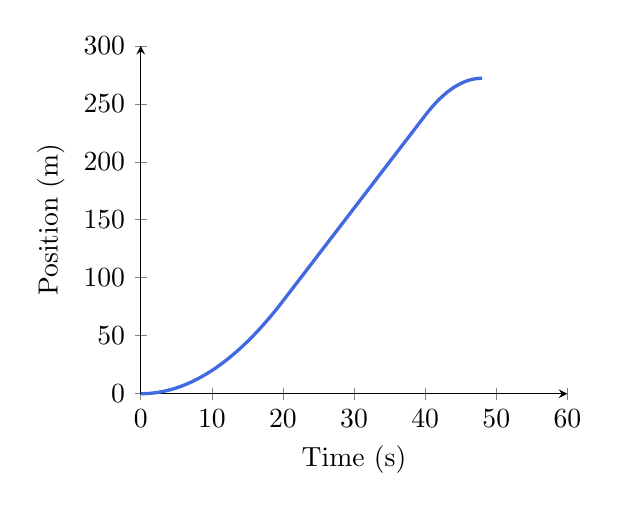
\begin{tikzpicture}
        \begin{axis}[width=7cm,
            height=6cm,
            axis lines=left,
            ylabel={Position (m)},
            xlabel={Time (s)},
            ymin=0,ymax=300,
            xmin=0,xmax=60,
            ytick={0,50,...,300},
            xtick={0,10,...,60},
            clip=false,
            ]
            \draw[very thick,RoyalBlue] plot[domain=0:20,samples=50,variable=\x] (\x,0.5*0.4*\x^2);
            \draw[very thick,RoyalBlue] plot[domain=20:40,samples=50,variable=\x] (\x,8*\x-80);
            \draw[very thick,RoyalBlue] plot[domain=40:48,samples=50,variable=\x] (\x,{-80+8*\x-0.5*(\x-40)^2});
        \end{axis}
    \end{tikzpicture}

    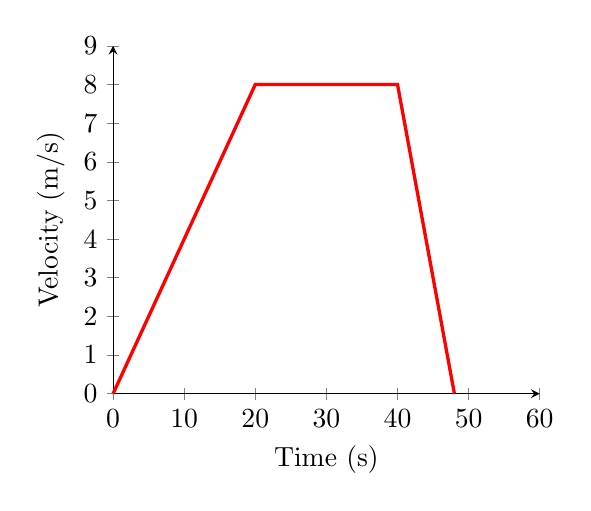
\begin{tikzpicture}
        \begin{axis}[width=7cm,
            height=6cm,
            axis lines=left,
            ylabel={Velocity (m/s)},
            xlabel={Time (s)},
            ymin=0,ymax=9,
            xmin=0,xmax=60,
            ytick={0,1,...,9},
            xtick={0,10,...,60},
            clip=false,
            ]
            \addplot[very thick,red,mark=none]
                coordinates{
                    (0,0)(20,8)(40,8)(48,0)
                };
        \end{axis}
    \end{tikzpicture}
    
    \begin{tikzpicture}
        \begin{axis}[width=7cm,
            height=6cm,
            axis lines=center,
            ylabel={Acceleration (\SI{}{m/s^2})},
            y label style={at={(axis description cs:0,1.05)}},
            xlabel={Time (s)},
            x label style={at={(axis description cs:0.65,-0.1)}},
            ymin=-1.2,ymax=0.6,
            xmin=0,xmax=60,
            ytick={-1.2,-1,...,0.6},
            xtick={0,10,...,60},
            clip=false,
            ]
            \addplot[very thick,Green,mark=none]
                coordinates{
                    (0,0.4)(20,0.4)(20,0)(40,0)(40,-1)(48,-1)
                };
        \end{axis}
    \end{tikzpicture}
    \captionsetup{type=figure,margin=1in,font=scriptsize}
    \captionof{figure}{(a) Position of the train over time. Notice that the train's position changes slowly at the beginning of the journey, then more and more quickly as it picks up speed. Its position then changes more slowly as it slows down at the end of the journey. In the middle of the journey, while the velocity remains constant, the position changes at a constant rate. (b) Velocity of the train over time. The train's velocity increases as it accelerates at the beginning of the journey. It remains the same in the middle of the journey (where there is no acceleration). It decreases as the train decelerates at the end of the journey. (c) The acceleration of the train over time. The train has positive acceleration as it speeds up at the beginning of the journey. It has no acceleration as it travels at constant velocity in the middle of the journey. Its acceleration is negative as it slows down at the end of the journey.}
    \label{RfUcWn}
\end{center}

\begin{example}
    \textit{Calculating Average Velocity: The Subway Train}. What is the average velocity of the train in part b of Example \ref{Zg8Ig4} if it takes \SI{5.00}{min} to make its trip? (See Figure \ref{GMa3RN}(b) for the picture.)
\end{example}

\Solution Recall that, by Equation \eqref{yHaY2u}, average velocity is displacement divided by time. It will be negative here, since the train moves to the left and has a negative displacement.

\vspace{1em}

We are given the initial and final positions and the elapsed time: $x_0^{\prime} = \SI{5.25}{km}$, $x_f^{\prime} = \SI{3.75}{km}$, and $\Delta t = \SI{5.00}{min}$. Also, we found displacement to be $\Delta x^{\prime} = -\SI{1.5}{km}$ in Example \ref{Zg8Ig4}. 

\vspace{1em}

Average velocity is

\begin{equation*}
    \bar{v} = \frac{\Delta x^{\prime}}{\Delta t} = \frac{-\SI{1.5}{km}}{\SI{5.00}{min}} 
\end{equation*}

We covert units as follows:

\begin{equation*}
    \bar{v} = \frac{\Delta x^{\prime}}{\Delta t} = \left(\frac{-\SI{1.5}{km}}{\SI{5.00}{min}}\right)
        \left(\frac{\SI{60}{min}}{\SI{1}{h}}\right) = -\SI{18}{km/h}
\end{equation*}

The negative velocity indicates motion to the left.

\endsolution

\begin{example} \label{2453yE}
    \textit{Calculating Deceleration: The Subway Train}. Finally, suppose the train in Figure \ref{GMa3RN}(b) slows to a stop from a velocity of \SI{20.0}{km/h} in \SI{10.0}{s}. What is its average acceleration?
\end{example}

\Solution Once again, let's draw a sketch:

\begin{center}
    \begin{tikzpicture}
        \begin{axis}[width=4cm,
            height=4cm,
            xmin=0,xmax=2,
            ymin=0,ymax=2,
            ticks=none,
            axis line style={draw=none},
            clip=false
            ]
            
            \draw[thick,->] (0,0) -- (1,0) node[right] {$x$};
            \draw[thick,->] (0,0) -- (0,1) node[above] {$y$};

            \begin{scope}[shift={(axis direction cs: -6,1)}]
                \draw[fill=black] (0,0.5) circle (2pt) node[below=2pt]{$v_f = \SI{0}{km/h}$};
                \draw (0,-0.5) node {\large \StopWatchEnd} node[below=3mm] {\SI{10.0}{s}};
                \draw[thick,<-] (1.5,0.5) -- ++(axis direction cs: 3,0) node[pos=0.5,below=2pt] {$v_0 = -\SI{20}{km/h}$}; 
                \draw (3,-0.5) node {\large \StopWatchStart} node[below=3mm] {\SI{0.0}{s}};
                \draw[Green,very thick,->] (0,-1.7) -- ++(axis direction cs: 3,0) node[pos=0.5,above] {$a =\ ?$};
            \end{scope}
        \end{axis}
    \end{tikzpicture}
\end{center}

As before, we must find the change in velocity and the change in time to calculate average acceleration.

\vspace{1em}

We are given initial velocity, final velocity, and elapsed time: $v_0 = -\SI{20}{km/h}$, $v_f = \SI{0}{km/h}$, and $\Delta t = \SI{10.0}{s}$. Next, we calculate $\Delta v$. The change in velocity here is actually positive, since

\begin{equation*}
    \Delta v = v_f - v_0 = 0 - \left(-\SI{20}{km/h}\right) = +\SI{20}{km/h}
\end{equation*}

Finally we solve for $\bar{a}$. By Equation \ref{vdyjX5}, average acceleration is

\begin{equation*}
    \bar{a} = \frac{\Delta v}{\Delta t} = \frac{+\SI{20}{km/h}}{\SI{10.0}{s}}
\end{equation*}

We convert units as follows:

\begin{equation*}
    \bar{a} = \left(\frac{+\SI[per-mode=fraction]{20}{\kilo\meter\per\hour}}{\SI{10.0}{s}}\right)
        \left(\frac{10^3\,\text{m}}{\SI{1}{km}}\right)\left(\frac{\SI{1}{h}}{\SI{3600}{s}}\right) = +\SI{0.556}{m/s^2}
\end{equation*}

The plus sign means that acceleration is to the right. This is reasonable because the train initially has a negative velocity (to the left) in this problem and a positive acceleration opposes the motion (and so it is to the right). Again, acceleration is in the same direction as the change in velocity, which is positive here. As in Example \ref{dHBSwG}, this acceleration can be called a deceleration since it is in the direction opposite to the velocity.

\endsolution

\subsubsection*{Sign and Direction}

Perhaps the most important thing to note about these examples is the signs of the answers. In our chosen coordinate system, plus means the quantity is to the right and minus means it is to the left. This is easy to imagine for displacement and velocity. But it is a little less obvious for acceleration. Most people interpret negative acceleration as the slowing of an object. This was not the case in Example \ref{2453yE}, where a positive acceleration slowed a negative velocity. The crucial distinction was that the acceleration was in the opposite direction from the velocity. In fact, a negative acceleration will increase a negative velocity. For example, the train moving to the left in Figure \ref{GMa3RN}(b) is sped up by an acceleration to the left. In that case, both $v$ and $a$ are negative. The plus and minus signs give the directions of the accelerations. If acceleration has the same sign as the velocity, the object is speeding up. If acceleration has the opposite sign as the velocity, the object is slowing down.

\subsection{Motion Equations for Constant Acceleration in One Dimension} \label{WbwyTy}

We might know that the greater the acceleration of, say, a car moving away from a stop sign, the greater the displacement in a given time. But we have not developed a specific equation that relates acceleration and displacement. In this section, we develop some convenient equations for kinematic relationships, starting from the definitions of displacement, velocity, and acceleration already covered.

\subsection*{Notation: $t$, $x$, $v$, $a$}

First, let us make some simplifications in notation. Taking the initial time to be zero, as if time is measured with a stopwatch, is a great simplification. Since elapsed time is $\Delta t = t_f - t_0$, taking $t_0 = 0$ means that $\Delta t = t_f$, the final time on the stopwatch. When initial time is taken to be zero, we use the subscript 0 to denote initial values of position and velocity. That is, $x_0$ \textit{is the initial position} and $v_0$ \textit{is the initial velocity}. We put no subscripts on the final values. That is, $t$ \textit{is the final time}, $x$ \textit{is the final position}, and $v$ \textit{is the final velocity}. This gives a simpler expression for elapsed time---now, $\Delta t = t$. It also simplifies the expression for displacement, which is now $\Delta x = x - x_0$. Also, it simplifies the expression for change in velocity, which is now $\Delta v = v - v_0$. To summarize, using the simplified notation, with the initial time taken to be zero,

\begin{align} \label{sclrF2}
    \Delta t &= t\\[0.5ex]
    \Delta x &= x - x_0\\[0.5ex]
    \Delta v &= v - v_0
\end{align}

where \textit{the subscript 0 denotes an initial value and the absence of a subscript denotes a final value} in whatever motion is under consideration.

\vspace{1em}

We now make the important assumption that \textit{acceleration is constant}. This assumption allows us to avoid using calculus to find instantaneous acceleration. Since acceleration is constant, the average and instantaneous accelerations are equal. That is,

\begin{equation}
    \bar{a} = a = \text{constant}
\end{equation}

so we use the symbol $a$ for acceleration at all times. Assuming acceleration to be constant does not seriously limit the situations we can study nor degrade the accuracy of our treatment. For one thing, acceleration is constant in a great number of situations. Furthermore, in many other situations we can accurately describe motion by assuming a constant acceleration equal to the average acceleration for that motion. Finally, in motions where acceleration changes drastically, such as a car accelerating to top speed and then braking to a stop, the motion can be considered in separate parts, each of which has its own constant acceleration.

\vspace{1em}

\cyanhrule

\begin{center}
\texttt{Solving for displacement ($\Delta x$) and final position ($x$) from average velocity when acceleration ($a$) is constant}
\end{center}

To get our first two new equations, we start with the definition of average velocity (Equation \ref{yHaY2u}): 

\begin{equation*}
    \bar{v} = \frac{\Delta x}{\Delta t}
\end{equation*}

Substituting the simplified notation for $\Delta{x}$ and $\Delta{t}$ from Equations \eqref{sclrF2} yields 

\begin{equation*}
    \bar{v} = \frac{x - x_0}{t}
\end{equation*}

Solving for $x$ yields 

\begin{equation} \label{FokTWv}
    x = x_0 + \bar{v}t
\end{equation}

where the average velocity is

\begin{equation}
    \bar{v} = \frac{v_0 + v}{2} \qquad \text{(constant $a$)}
\end{equation}

\cyanhrule

\vspace{1em}

Equation \eqref{robof8}, $\bar{v} = \frac{v_0 + v}{2}$, reflects the fact that, when acceleration is constant, $v$ is just the simple average of the initial and final velocities. For example, if you steadily increase your velocity (that is, with constant acceleration) from 30 to \SI{60}{km/h}, then your average velocity during this steady increase is \SI{45}{km/h}. Using Equation \eqref{robof8} to check this, we see that 

\begin{equation*}
    \bar{v} = \frac{v_0 + v}{2} = \frac{\SI[per-mode=fraction]{30}{\kilo\meter\per\hour} + \SI[per-mode=fraction]{60}{\kilo\meter\per\hour}}{2} = \SI{45}{km/h}
\end{equation*}

which seems logical.

\begin{example}
    \textit{Calculating Displacement: How Far does the Jogger Run?} A jogger runs down a straight stretch of road with an average velocity of \SI{4.00}{m/s} for \SI{2.00}{min}. What is his final position, taking his initial position to be zero?
\end{example}

\Solution Let's draw a sketch.

\begin{center}
    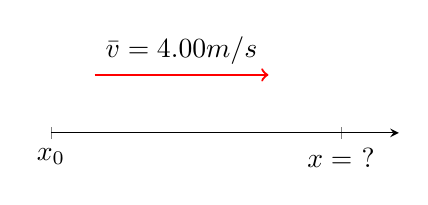
\begin{tikzpicture}
        \begin{axis}[
            width=6cm,
            height=6cm,
            xmin=0,xmax=12,
            ymin=0,ymax=12,
            axis x line=left,
            axis y line=none,
            ytick=\empty,
            clip=false,
            xtick={0,10}, 
            xticklabels = {$x_0$, $x =\ ?$}, 
        ]

        \draw[red,thick,->] (1.5,2) -- ++(6,0) node[pos=0.5,above,black] {$\bar{v} = \SI{4.00}{m/s}$};
        \end{axis}
        \hspace{6cm}
        \begin{axis}[
            width=2.4cm,
            height=2.4cm,
            xmin=0,xmax=1,
            ymin=0,ymax=1,
            axis lines=center,
            ticks=none,
            xlabel={$x$},
            ylabel={$y$},
        ]
        \end{axis}
    \end{tikzpicture}
\end{center}

The final position $x$ is given by Equation \eqref{FokTWv} as

\begin{equation*}
    x = x_0 + \bar{v} t
\end{equation*}

To find $x$, we identify the values of $x_0$, $\bar{v}$, and $t$, from the statement of the problem and substitute them into the equation.

\vspace{1em}

We are given average velocity, elapsed time, and initial position: 

\begin{equation*}
    \bar{v} = \SI{4.00}{m/s}\ , \quad \Delta t = \SI{2.00}{min}\ , \quad x_0 = 0
\end{equation*}

Substituting the given values into Equation \eqref{FokTWv} leads to 

\begin{equation*}
    x = x_0 + \bar{v} t = 0 + \left(\SI{4.00}{m/s}\right) \left(\SI{120}{s}\right) = \SI{480}{m}
\end{equation*}

Velocity and final displacement are both positive, which means they are in the same direction.

\endsolution

Equation \eqref{FokTWv}, $x = x_0 + \bar{v} t$, gives insight into the relationship between displacement, average velocity, and time. It shows, for example, that displacement is a linear function of average velocity. (By linear function, we mean that displacement depends on $\bar{v}$ rather than on $\bar{v}$ raised to some other power, such as $\bar{v}^2$. When graphed, linear functions look like straight lines with a constant slope.) On a car trip, for example, we will get twice as far in a given time if we average \SI{90}{km/h} than if we average \SI{45}{km/h}.


\begin{center}
    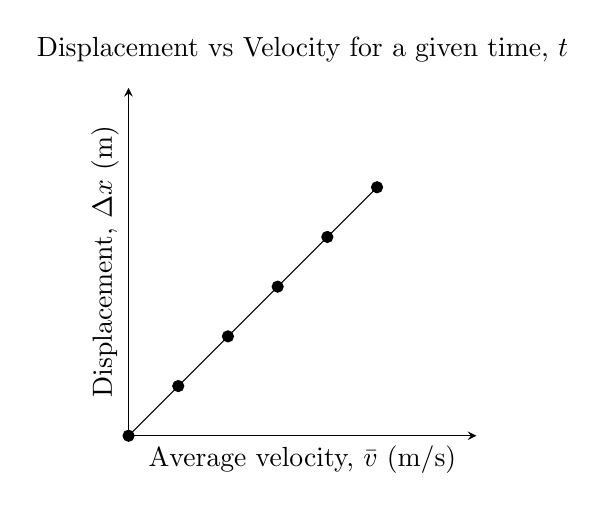
\begin{tikzpicture}
        \begin{axis}[axis lines=left,
            width=6cm,
            height=6cm,
            ticks=none,
            ylabel={Displacement, $\Delta x$ (m)},
            xlabel={Average velocity, $\bar{v}$ (m/s)},
            title={Displacement vs~Velocity for a given time, $t$},
            xmin=0,xmax=7,
            ymin=0,ymax=7,
        ]
        \addplot[black,mark=*]
            coordinates{
                (0,0)(1,1)(2,2)(3,3)(4,4)(5,5)
            };
        \end{axis}
    \end{tikzpicture}
\captionsetup{type=figure,margin=1in,font=scriptsize}
\captionof{figure}{There is a linear relationship between displacement and average velocity. For a given time $t$, an object moving twice as fast as another object will move twice as far as the other object.}
\end{center}

\cyanhrule

\begin{center}
   \texttt{Solving for final velocity} 
\end{center}

We can derive another useful equation by manipulating the definition of acceleration, Equation \eqref{vdyjX5}.

\begin{equation*}
    a = \frac{\Delta v}{\Delta t}
\end{equation*}

Substituting the simplified notation for $\Delta v$ and $\Delta t$ give us

\begin{equation*}
    a = \frac{v - v_0}{t}
\end{equation*}

Solving for $v$ yields

\begin{equation} \label{0bbOYZ}
    v = v_0 + a t
\end{equation}

\cyanhrule

\vspace{1em}

\begin{example}
    \textit{Calculating Final Velocity: An Airplane Slowing Down after Landing}. An airplane lands with an initial velocity of \SI{70.0}{m/s} and then decelerates at \SI{1.50}{m/s^2} for \SI{40.0}{s}. What is its final velocity?
\end{example}

\Solution Draw a sketch. We draw the acceleration vector in the direction opposite the velocity vector because the plane is decelerating.


\begin{center}
    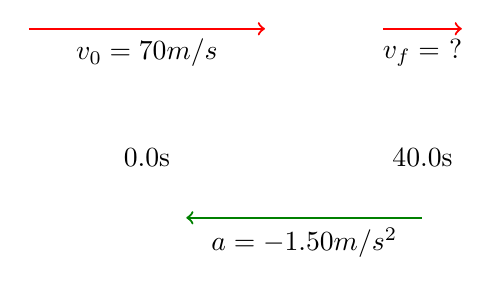
\begin{tikzpicture}
        \draw[thick,red,->] (0,1.2) -- ++(3,0) node[black,below,pos=0.5] {$v_0 = \SI{70}{m/s}$};
        \draw[thick,red,->] (4.5,1.2) -- ++(1,0) node[black,below,pos=0.5] {$v_f =\ ?$};
        \draw (1.5,0) node{\large \StopWatchStart} node[below=2mm] {\SI{0.0}{s}};
        \draw (5,0) node{\large \StopWatchEnd} node[below=2mm] {\SI{40.0}{s}};
        \draw[<-,thick,Green] (2,-1.2) -- ++(3,0) node[below,pos=0.5,black] {$a=-\SI{1.50}{m/s^2}$};
        \hspace{8cm}
        \begin{axis}[width=2.4cm,
            height=2.4cm,
            ticks=none,
            axis lines=center,
            ylabel=$y$,
            xlabel=$x$
        ]
        \end{axis}
    \end{tikzpicture}
\end{center}

1. Identify the knowns. We are given initial velocity, acceleration, and time: $v_0 = \SI{70.0}{m/s}$, $a = -\SI{1.50}{m/s^2}$, and $t = \SI{40.0}{s}$. 

\vspace{1ex}

2. Identify the unknown. In this case, it is final velocity, $v_f$.

\vspace{1ex}

3. Determine which equation to use. We can calculate the final velocity using Equation \eqref{0bbOYZ}:

\begin{equation*}
    v = v_0 + at
\end{equation*}

4. Plug in the known values and solve.

\begin{equation*}
    v = v_0 + at = \SI{70.0}{m/s} + \left(-\SI{1.50}{m/s^2}\right)\left(\SI{40.0}{s}\right) = \SI{10.0}{m/s}
\end{equation*}

The final velocity is much less than the initial velocity, as desired when slowing down, but still positive. With jet engines, reverse thrust could be maintained long enough to stop the plane and start moving it backward. That would be indicated by a negative final velocity, which is not the case here.

\endsolution 

In addition to being useful in problem solving, the equation \eqref{0bbOYZ} $v = v_0 + at$ gives us insight into the relationships among velocity, acceleration, and time. From it we can see, for example, that

\begin{itemize}
    \item final velocity depends on how large the acceleration is and how long it lasts
    \item if the acceleration is zero, then the final velocity equals the initial velocity ($v=v_0$), as expected (i.e., velocity is constant)
    \item if $a$ is negative, then the final velocity is less than the initial velocity
\end{itemize}

(All of these observations fit our intuition, and it is always useful to examine basic equations in light of our intuition and experiences to check that they do indeed describe nature accurately.)

% Skip MAKING CONNECTIONS: REAL-WORLD CONNECTION

\vspace{1em}

\cyanhrule

\begin{center}
    \texttt{SOLVING FOR FINAL POSITION WHEN VELOCITY IS NOT CONSTANT} ($a \neq 0 $)
\end{center}


We can combine the equations above to find a third equation that allows us to calculate the final position of an object experiencing constant acceleration. We start with Equation \eqref{0bbOYZ}:

\begin{equation*}
    v = v_0 + a t
\end{equation*}

Adding $v_0$ to each side of this equation and dividing by 2 gives

\begin{equation*}
    \frac{v_0 + v}{2} = v_0 + \frac{1}{2} a t
\end{equation*}

Since

\begin{equation*}
    \frac{v_0 + v}{2} = \bar{v}
\end{equation*}

for constant acceleration, then 

\begin{equation*}
    \bar{v} = v_0 + \frac{1}{2} a t^2 
\end{equation*}

Now we substitute this expression for $\bar{v}$ into the equation for displacement, Equation \eqref{FokTWv}, $x = x_0 + \bar{v} t$, yielding

\begin{equation} \label{03Tfzm}
    x = x_0 + v_0 t + \frac{1}{2} a t^2
\end{equation}

which assumes constant $a$.

\vspace{1em}

\cyanhrule

\begin{example} \label{7ddBPA}
    \textit{Calculating Displacement of an Accelerating Object: Dragsters}. Dragsters can achieve average accelerations of \SI{26.0}{m/s^2}. Suppose such a dragster accelerates from rest at this rate for \SI{5.56}{s}. How far does it travel in this time?
\end{example}

\Solution Draw a sketch.

\begin{center}
    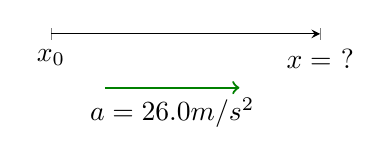
\begin{tikzpicture}
        \begin{axis}[width=5cm,height=5cm,
            xmin=0,xmax=10,
            ymin=0,ymax=10,
            axis y line=none,
            axis x line=left,
            clip=false,
            xtick={0,10},
            xticklabels={$x_0$,$x=\ ?$},
        ]
        \draw[->,thick,Green] (2,-2) -- ++ (5,0) node[black,below,pos=0.5] {$a = \SI{26.0}{m/s^2}$};
        \end{axis}
        \hspace{5cm}
        \xydirection
    \end{tikzpicture}
\end{center}

We are asked to find displacement, which is $x$ if we take $x_0$ to be zero. (Think about it like the starting line of a race. It can be anywhere, but we call it 0 and measure all other positions relative to it.) We can use Equation \eqref{03Tfzm} $x = x_0 + v_0 t + \frac{1}{2} a t^2$ once we identify $v_0$, $a$, and $t$ from the statement of the problem.

\vspace{1em}

1. Identify the knowns. Starting from rest means that $v_0 = 0$, $a$ is given as $\SI{26.0}{m/s^2}$, and $t$ is given as \SI{5.56}{s}. 

\vspace{1em}

2. Plug the known values into the equation to solve for the unknown $x$. 

\begin{equation*}
    x = x_0 + v_0 t + \frac{1}{2} a t^2
\end{equation*}

Since the initial position and velocity are both zero, this simplifies to

\begin{equation*}
    x = \frac{1}{2} a t^2 
\end{equation*}

Substituting the identified values of $a$ and $t$ gives

\begin{equation*}
    x = \frac{1}{2}\left(\SI{26.0}{m/s^2}\right)\left(\SI{5.56}{s}\right)^2
\end{equation*}

yielding

\begin{equation*}
    x = \SI{402}{m}
\end{equation*}

\textbf{Discussion}: If we convert \SI{402}{m} to miles, we find that the distance covered is very close to one quarter of a mile, the standard distance for drag racing. So the answer is reasonable. This is an impressive displacement in only \SI{5.56}{s}, but top-notch dragsters can do a quarter mile in even less time than this.

\endsolution

\vspace{1em}

What else can we learn by examining the Equation \eqref{03Tfzm} $x = x_0 + v_0 t + \frac{1}{2} a t^2$ ? We see that:

\begin{itemize}
    \item displacement depends on the square of the elapsed time when acceleration is not zero. In Example \ref{7ddBPA}, the dragster covers only one fourth of the total distance in the first half of the elapsed time
    \item if acceleration is zero, then the initial velocity equals average velocity ($v_0 = \bar{v}$) and $x = x_0 + v_0 t + \frac{1}{2} a t^2$ (Eq.~\ref{03Tfzm}) becomes $x = x_0 + v_0 t$ (Eq.~\ref{FokTWv}).
\end{itemize}

\cyanhrule

\vspace{1em}

\texttt{SOLVING FOR FINAL VELOCITY WHEN VELOCITY IS NOT CONSTANT} ($a \neq 0 $)

\vspace{1em}

A fourth useful equation can be obtained from another algebraic manipulation of previous equations.

\vspace{1em}

If we solve $v = v_0 + a t$ (Equation \ref{0bbOYZ}) for $t$ , we get

\begin{equation*}
    t = \frac{v - v_0}{a} 
\end{equation*}

Substituting this and $\bar{v} = \frac{v_0 + v}{2}$ into $x = x_0 + \bar{v} t$, we get 

\begin{equation} \label{jIcda3}
    v^2 = v_0^2 + 2 a (x-x_0)
\end{equation}

\cyanhrule

\vspace{1em}

\begin{example}
    \textit{Calculating Final Velocity: Dragsters}. Calculate the final velocity of the dragster in Example \ref{7ddBPA} without using information about time.
\end{example}

\Solution We draw the same sketch.

\begin{center}
    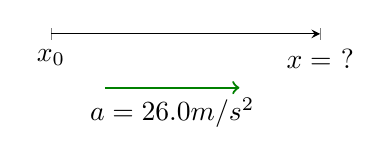
\begin{tikzpicture}
        \begin{axis}[width=5cm,height=5cm,
            xmin=0,xmax=10,
            ymin=0,ymax=10,
            axis y line=none,
            axis x line=left,
            clip=false,
            xtick={0,10},
            xticklabels={$x_0$,$x=\ ?$},
        ]
        \draw[->,thick,Green] (2,-2) -- ++ (5,0) node[black,below,pos=0.5] {$a = \SI{26.0}{m/s^2}$};
        \end{axis}
        \hspace{5cm}
        \xydirection
    \end{tikzpicture}
\end{center}

The equation \eqref{jIcda3} $v^2 = v_0^2 + 2a(x-x_0)$ is ideally suited to this task because it relates velocities, acceleration, and displacement, and no time information is required.

\vspace{1em}

1. Identify the known values. We know that $v_0 = 0$, since the dragster starts from rest. Then we note that $x - x_0 = \SI{402}{m}$ (this was the answer in Example \ref{7ddBPA}). Finally, the average acceleration was given to be $a=\SI{26.0}{m/s^2}$.

\vspace{1em}

2. Plug the knowns into the equation \eqref{jIcda3} $v^2 = v_0^2 + 2a(x-x_0)$ and solve for $v$. 

\begin{equation*}
    v^2 = 0 + 2\left(\SI{26.0}{m/s^2})\right)\left(\SI{402}{m}\right)
\end{equation*}

Thus

\begin{equation*}
    v^2 = \SI{2.09e4}{m^2/s^2}
\end{equation*}

To get $v$, we take the square root

\begin{equation*}
    v = \sqrt{\SI{2.09e4}{m^2/s^2}} = \SI{145}{m/s}
\end{equation*}

\textbf{Discussion}: \SI{145}{m/s} is about \SI{522}{km/h} or about \SI{324}{mi/h}, but even this breakneck speed is short of the record for the quarter mile. Also, note that a square root has two values; we took the positive value to indicate a velocity in the same direction as the acceleration.

\endsolution

\vspace{1em}

An examination of the equation $v^2 = v_0^2 + 2a(x-x_0)$ can produce further insights into the general relationships among physical quantities:

\begin{itemize}
    \item The final velocity depends on how large the acceleration is and the distance over which it acts
    \item For a fixed deceleration, a car that is going twice as fast doesn't simply stop in twice the distance---it takes much further to stop. (This is why we have reduced speed zones near schools.)
\end{itemize}

\subsection*{Putting Equations Together}

In the following examples, we further explore one-dimensional motion, but in situations requiring slightly more algebraic manipulation. The examples also give insight into problem-solving techniques. The box below provides easy reference to the equations needed.

\vspace{1em}

\cyanhrule

\begin{center}
    \texttt{SUMMARY OF KINEMATIC EQUATIONS (CONSTANT $a$)}
\end{center}

\vspace{-2em}

\begin{align}
    x &= x_0 + \bar{v} t \label{X0SPQW} \\[1ex]
    \bar{v} &= \frac{v_0 + v}{2} \\[1ex]
    v &= v_0 + at \\[1ex]
    x &= x_0 + v_0t + \frac{1}{2} a t^2 \label{eo2SPc} \\[1ex]
    v^2 &= v_0^2 + 2a (x - x_0) \label{EEJoew}
\end{align}

\cyanhrule

\begin{example}
    \textit{Calculating Displacement: How Far Does a Car Go When Coming to a Halt?} On dry concrete, a car can decelerate at a rate of \SI{7.00}{m/s^2}, whereas on wet concrete it can decelerate at only \SI{5.00}{m/s^2}. Find the distances necessary to stop a car moving at \SI{30.0}{m/s} (about \SI{110}{km/h}) (a) on dry concrete and (b) on wet concrete. (c) Repeat both calculations, finding the displacement from the point where the driver sees a traffic light turn red, taking into account his reaction time of \SI{0.500}{s} to get his foot on the brake.
\end{example}

\Solution Draw a sketch.

\begin{center}
    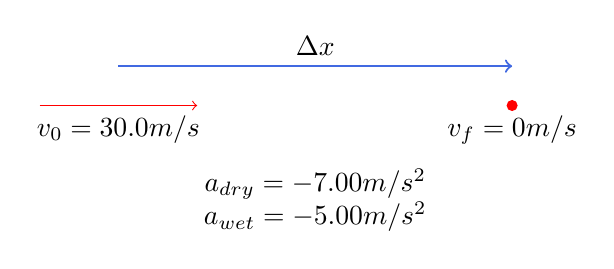
\begin{tikzpicture}
        \draw[->,RoyalBlue,thick] (0,0) -- ++(5,0) node[above,pos=0.5,black] {$\Delta x$};
        \draw[->,red] (-1,-0.5) -- ++(2,0) node[below,pos=0.5,black] {$v_0 = \SI{30.0}{m/s}$};
        \fill[red] (5,-0.5) circle (2pt) node[below,black] {$v_f = \SI{0}{m/s}$};
        \draw (2.5,-1.5) node {$a_{\text{dry}} = -\SI{7.00}{m/s^2}$} 
            node[below=3pt] {$a_{\text{wet}} = -\SI{5.00}{m/s^2}$};
    \end{tikzpicture}
\end{center}

In order to determine which equations are best to use, we need to list all of the known values and identify exactly what we need to solve for. We shall do this explicitly in the next several examples, using tables to set them off.

\vspace{1em}

(a) Let's identify the knowns and what we want to solve for. We are given initial velocity, final velocity, and acceleration: $v_0 = \SI{30.0}{m/s}$, $v= 0$, and $a = \SI{-7.00}{m/s^2}$ ($a$ is negative because it is in a direction opposite to velocity). Also, we take $x_0$ to be zero. The unknown we are looking for is displacement: $\Delta x$, or $x-x_0$.

\vspace{1em}

Next, we identify the equation that will help up solve the problem. The best equation to use is Equation \eqref{EEJoew}:

\begin{equation*}
    v^2 = v_0^2 + 2a(x-x_0)
\end{equation*}

This equation is best because it includes only one unknown, $x$. We know the values of all the other variables in this equation. (There are other equations that would allow us to solve for $x$, but they require us to know the stopping time, $t$, which we do not know. We could use them but it would entail additional calculations.)

\vspace{1em}

Substituting known values into Equation \eqref{EEJoew} (and omitting units) leads to 

\begin{equation*}
    0^2 = 30^2 + 2\left(-7\right) \left(x-0\right)
\end{equation*}

or, more simply, to 

\begin{equation*}
    0 = 30^2 - 14 x
\end{equation*}

Now we can rearrange the equation to solve for $x$, as follows:

\begin{align*}
    \textbf{Add $14x$} \qquad & 0 \redplus \textcolor{red}{14x} = 30^2 -14x \redplus \textcolor{red}{14x}\\[1ex]
    \textbf{Simplify} \qquad & 14x = 30^2\\[1ex]
    \textbf{Divide by 14} \qquad & \frac{\cancel{14}x}{\textcolor{red}{\cancel{14}}} = \frac{30^2}{\textcolor{red}{14}}\\[1ex]
    \textbf{Simplify} \qquad & x = \frac{30^2}{14} \\[1ex]
    \textbf{Compute} \qquad & x = 64.3
\end{align*}

Therefore, displacement is $x = \SI{64.3}{m}$ on dry concrete.

\vspace{1em}

(b) This part can be solved in exactly the same manner as Part A. The only difference is that the deceleration is $-\SI{5.00}{m/s^2}$. The result is $x = \SI{90.0}{m}$ on wet concrete.

\vspace{1em}

(c) Once the driver reacts, the stopping distance is the same as it is in Parts A and B for dry and wet concrete. So to answer this question, we need to calculate how far the car travels during the reaction time, and then add that to the stopping time. It is reasonable to assume that the velocity remains constant during the driver’s reaction time.

\vspace{1em}

We identify the knowns and what we want to solve for. We are given average velocity, reaction time, and acceleration during reaction: $\bar{v} = \SI{30}{m/s}$, $t_{\text{reaction}} = \SI{0.500}{m/s}$, and $a_{\text{reaction}} = 0$.  We take $x_{0,\text{reaction}}$ to be 0. We are looking for $x_{\text{reaction}}$. 

\vspace{1em} 

Now we identify the best equation to use. Equation \eqref{X0SPQW}, $x = x_0 + \bar{v} t$, works well because the only unknown value is $x$, which is what we want to solve for. 

\vspace{1em}

Substituting given values leads to 

\begin{equation*}
    x = x_0 + \bar{v} t = 0 + \left(\SI{30.0}{m/s}\right) \left(\SI{0.500}{s}\right) = \SI{15.0}{m}
\end{equation*}

This means the car travels 15.0 meters while the driver reacts, making the total displacements in the two cases of dry and wet concrete \SI{15.0}{m} greater than if he reacted instantly.

\vspace{1em}

Add the displacement during the reaction time to the displacement when braking:

\begin{align*}
    x_{\text{braking}} + x_{\text{reaction}} &= x_{\text{final}}\\[1ex]
    \SI{64.3}{m} + \SI{15.0}{m} &= \SI{79.3}{m} \quad \text{when dry}\\
    \SI{90.0}{m} + \SI{15.0}{m} &= \SI{105}{m} \quad \text{when wet}
\end{align*}

\textbf{Discussion}: The displacements found in this example seem reasonable for stopping a fast-moving car. It should take longer to stop a car on wet rather than dry pavement. It is interesting that reaction time adds significantly to the displacements. But more important is the general approach to solving problems. We identify the knowns and the quantities to be determined and then find an appropriate equation. There is often more than one way to solve a problem. The various parts of this example can in fact be solved by other methods, but the solutions presented above are the shortest.

\endsolution

\begin{example}
    \textit{Calculating Time: A Car Merges into Traffic}. Suppose a car merges into freeway traffic on a 200-m-long ramp. If its initial velocity is 10.0 m/s and it accelerates at \SI{2.00}{m/s^2}, how long does it take to travel the 200 m up the ramp? (Such information might be useful to a traffic engineer.)
\end{example}

\Solution Draw a sketch.

\begin{center}
    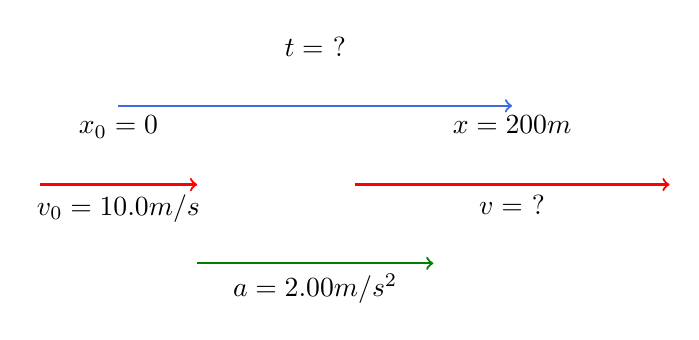
\begin{tikzpicture}
        \draw[->,thick,RoyalBlue] (0,0) node[below,black] {$x_0 = 0$} -- ++(5,0) node[below,black] {$x = \SI{200}{m}$} node[black,pos=0.5,above=5mm] {$t=\ ?$};
        \draw[->,red,thick] (-1,-1) -- ++(2,0) node[pos=0.5,below,black] {$v_0 = \SI{10.0}{m/s}$}; 
        \draw[->,red,thick] (3,-1) -- ++(4,0) node[pos=0.5,below,black] {$v =\ ?$};
        \draw[->,Green,thick] (1,-2) -- ++(3,0) node[pos=0.5,below,black] {$a = \SI{2.00}{m/s^2}$};
    \end{tikzpicture}
\end{center}

We are asked to solve for the time $t$. As before, we identify the known quantities in order to choose a convenient physical relationship (that is, an equation with one unknown, $t$).

\vspace{1em}

We identify the givens and what we want to solve for. We know initial velocity, acceleration, and displacement: $v_0 = \SI{10}{m/s}$, $a = \SI{2.00}{m/s^2}$, $x = \SI{200}{m}$. 

\vspace{1em}

We need to solve for time: $t =\ ?$ Choose the best equation. Equation \eqref{eo2SPc}, $x = x_0 + v_0 t + \frac{1}{2} a t^2$, works best because the only unknown in the equation is the variable $t$ for which we need to solve.

\vspace{1em}

We will need to rearrange the equation to solve for $t$. It will be easier to plug in the knowns first. Substituting known values leads to 

\begin{equation*}
    \SI{200}{m} = \SI{0}{m} + \left(\SI{10}{m/s}\right) t + \frac{1}{2}\left(\SI{2.00}{m/s^2}\right) t^2
\end{equation*}

Simplify the equation. The units of meters (m) cancel because they are in each term. We can get the units of seconds (s) to cancel by taking  $t = t\,\text{s}$, where $t$ is the magnitude of time and s is the unit. Doing so leaves

\begin{equation*}
    200 = 10t + t^2
\end{equation*}

Next, we use the quadratic formula to solve for $t$. We rearrange the equation to get 0 on one side of the equation, as follows:

\begin{align*}
    \textbf{Swap equation sides} \qquad & t^2 + 10t = 200\\[1ex]
    \textbf{Subtract 200} \qquad & t^2 + 10t \redminus \textcolor{red}{200} = 200 \redminus \textcolor{red}{200}\\[1ex]
    \textbf{Simplify} \qquad & t^2 + 10t - 200 = 0
\end{align*}

This equation

\begin{equation} \label{uIBlB1}
    t^2 + 10t - 200 = 0
\end{equation}

is a quadratic equation of the form

\begin{equation}
    a t^2 + bt + c = 0
\end{equation}

where the constants are $a = 1.00$, $b = 10.0$, and $c = -200$. The solutions to Equation \eqref{uIBlB1} are given by the quadratic formula:

\begin{equation}
    t = \frac{-b \pm \sqrt{b^2 - 4ac}}{2a}
\end{equation}

This yields two solutions for $t$, which are

\begin{equation*}
    t = 10.0 \quad \text{and} \quad -20.0
\end{equation*}

In this case, then, the time is $t = t$ in seconds, or

\begin{equation*}
     t = \SI{10.0}{s} \quad \text{and} \quad -\SI{20.0}{s}
\end{equation*}

A negative value for time is unreasonable, since it would mean that the event happened \SI{20}{s} before the motion began. We can discard that solution. Thus,

\begin{equation*}
    t = \SI{10.0}{s}
\end{equation*}

\textbf{Discussion}: Whenever an equation contains an unknown squared, there will be two solutions. In some problems both solutions are meaningful, but in others, such as the above, only one solution is reasonable. The \SI{10.0}{s} answer seems reasonable for a typical freeway on-ramp.

\endsolution

\vspace{1em}

With the basics of kinematics established, we can go on to many other interesting examples and applications. In the process of developing kinematics, we have also glimpsed a general approach to problem solving that produces both correct answers and insights into physical relationships. ``Problem-Solving Basics'' discusses problem-solving basics and outlines an approach that will help you succeed in this invaluable task.


\clearpage

\subsection{Exercises}

\subsubsection*{\nameref{1QLrzP}} %Vectors, Scalars,...

\begin{exercise} \label{hJNNqd}
    A person's speed can stay the same as they round a corner and changes direction. Given this information, is speed a scalar or a vector quantity? Explain.
\end{exercise}

\subsubsection*{\nameref{LgXYss}} %Acceleration

\begin{exercise} \label{OKpKf5}
    An airplane lands on a runway traveling east. Describe its acceleration.
\end{exercise}

\subsubsection*{\nameref{WbwyTy}} %Motion Equations

\begin{exercise} \label{HbNHjj}
A rocket accelerates at a rate of \SI{20}{m/s^2} during launch. How long does it take the rocket to reach a velocity of \SI{400}{m/s}?
\end{exercise}

\subsection{Answers to Select Exercises}

\subsubsection*{\nameref{1QLrzP}} %Vectors, Scalars,...

\ref{hJNNqd}. Speed is a scalar quantity. It does not change at all with direction changes; therefore, it has magnitude only. If it were a vector quantity, it would change as direction changes (even if its magnitude remained constant).\\

\subsubsection*{\nameref{LgXYss}} %Acceleration

\ref{OKpKf5}. If we take east to be positive, then the airplane has negative acceleration, as it is accelerating toward the west. It is also decelerating: its acceleration is opposite in direction to its velocity.\\

\subsubsection*{\nameref{WbwyTy}} %Motion Equations
\ref{HbNHjj}. \SI{20}{s}\\

\end{document}